\chapter{Implementation}
\label{ch:implementation}
When the Coffee Time specification was created and the prototype was tested, the implementation itself could begin. In this chapter, the implementation details are covered. In the beginning, the proposed architecture of the application is introduced and explained. Next section describes how the Coffee Time API is designed and implemented. Which framework for creating REST API was chosen and how it can be connected to Firebase services. Detailed section of the mobile application implementation follows. In this section, used techniques and packages are described to achieve desired functionality. 
% ----- % ----- % ----- % ----- % ----- % ----- % ----- % ----- % ----- % ----- % ----- % ----- % ----- % ----- %
\section{Clean Architecture}
In order to have easy to write, maintainable and testable code, some overall architecture should be considered. The~architecture should follow these rules: 
\begin{enumerate}
\item Independence of \gls{ui} from application business logic. 
\item The business logic has to be testable without any dependent requirements such as server connections.
\item Interchangeable \gls{ui}. The \gls{ui} part can be changed without affecting the rest of the system.
\item Independence of business logic from the infrastructure -- the data source can be changed without affecting business logic.
\end{enumerate}

\begin{figure}[ht]
    \centering
    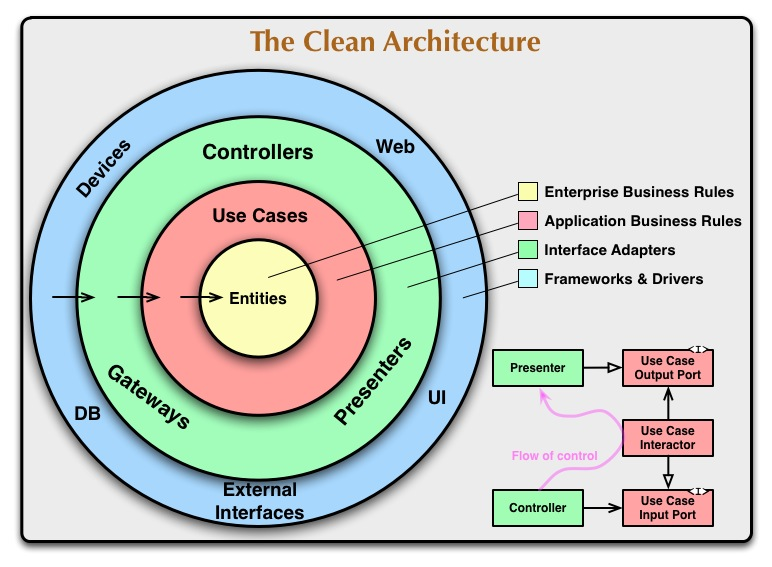
\includegraphics[width=0.75\linewidth]{img/implementation/CleanArchitecture.jpg}
    \caption{Clean Architecture defined by B.~Martin~\cite{clean-architecture-article}.}
    \label{fig:clean-arch-bmartin}
\end{figure}

There are several attempts and approaches on how to design such architecture~\cite{clean-architecture-article}. The inspiration for chosen architecture comes from Clean Architecture, initially proposed by \textit{Bob Martin}~\cite{clean-architecture-book}. In the basic form the clean architecture (\cref{fig:clean-arch-bmartin}) consists of four layers organised as circles. Architecture defines dependency rule where each layer should be dependent only on the inner circles. Accordingly to B. Martin~\cite{clean-architecture-article} layers can be described as:  

\begin{quote}
\textbf{Entities} encapsulate Enterprise-wide business rules. These entities, which can be simple objects or hierarchical structure of objects are the least likely to change when something external changes.

\textbf{Use Cases} are application-specific business rules. They encapsulate all of the use cases of the system. These use cases orchestrate the flow of data to and from the entities and direct those entities to use their enterprise-wide business rules to achieve the goals of the use case. Changes within the use case do not affect entities and similarly, changes of outer layers (such as interchanging database provider) do not affect the use cases. 

\textbf{Interface Adapters} converts data from the format most convenient for the use cases and entities to the format most convenient for some external agency such as database or API.  The application presentation (UI) should be here. Data models in this layer most likely consist only of data that are passed down to the use cases and then back from use cases to the view.  This layer is also responsible for converting any data from external forms into an internal form used by the use cases.

\textbf{Frameworks and Driver} contain any external frameworks and tools. This layer typically exposes interfaces to glue the external framework wit the rest of the application. 
\end{quote}

This architecture was chosen for its simplicity of dependencies, easy testability and extendability. 
% ----- % ----- % ----- % ----- % ----- % ----- % ----- % ----- % ----- % ----- % ----- % ----- % ----- % ----- %
\section{Coffee Time API}
The Coffee Time API is served through Firebase Cloud Functions services . Each function can run the backend code in response to events triggered by Firebase features and HTTPS requests. Functions can be written with JavaScript or Typescript language. For implementation, the Typescript was chosen due to the safer typing system, and due to the fact, that author has more experience with Typescript than with plain JavaScript. 

Functions are written under Node.js~\cite{node-js}, and every function that is exported is considered as ``Cloud function'' and can be accessed through HTTPS request. This can be used to build fully functional REST API. For the implementation, Express.js framework~\cite{express-js} was selected as popular and easy to use solution. Developers define routes, which HTTP method can be used and how the request should be processed. 
Express.js has a simple yet powerful mechanism of middlewares, where each request can be pre-processed before sending to the next processing. For example, it can be used to check if the user is authorised to make the request. With this setup, nothing prevented to create Coffee Time API. Furthermore, as~Express.js allows to define REST API, only one cloud function can be exported -- ``the api'' function. All requests are processed through this function. However, before implementation itself, it had to be defined what API will offer and how it can be consumed. 
% --- # --- # --- # --- # --- # --- # --- # --- # --- # --- # --- # --- # --- # --- # --- # --- # --- # --- #
\subsection{The API Endpoints}
The API has endpoints divided into three categories -- places, tags and photos. As a~client is considered to be multilingual, the API is too. The Places API accepts, as was described earlier, language parameter to specify how the response should be localised. The API is designed with language parameter as a mandatory part of the~URL for places related requests. The tags category has endpoints for obtaining and manipulating tags. Lastly, photo category gives access to downloading the place's photo. Every response coming from \gls{gpa} which returns places are modified such that each ``place'' entry contains additional \verb|tags| field which is an~array of the~\verb|tag| model. 

The~\cref{table:cta-places} describes each API endpoint and its usage. Mandatory parameters within the~URL are highlighted as \verb|<param>|. Each URL is shown without prefix \verb|http[s]://domain/api| (the hosting URL and \verb|/api| suffix).
% -----------------------------
\begin{table}[ht]
\centering
\begin{tabularx}{\textwidth}{|l|l|X|}
\hline
\textbf{URL} & \textbf{HTTP Method} & \textbf{Description} \\ \hline
\verb|<language>/nearby?parameters| & GET & Get nearby cafes \\ \hline
\verb|<language>/find?parameters| & GET & Find cafes within area based on text query \\ \hline
\verb|<language>/detail/<place_id>| & GET & Place's details of given \verb|place_id| \\ \hline
\verb|<language>/basic/<place_id>| & GET & Returns basic place information \\ \hline
\end{tabularx}
\caption{Places Endpoints.}
\label{table:cta-places}
\end{table}
% -----------------------------
\begin{table}[ht]
\centering
\begin{tabularx}{\textwidth}{|l|l|X|}
\hline
\textbf{Parameter} & \textbf{Required} & \textbf{Description} \\ \hline
\verb|location=lat,lng| & Yes & Location to search, where \verb|lat|=latitude, \verb|lng|=longitude \\ \hline
\verb|radius| & No & If omitted, the results is sorted by \textit{prominence} (see below), otherwise by distance\\ \hline
\verb|opennow| & No & If present returns only opened cafes\\ \hline
\verb|pagetoken| & No & If present, next page returned\\ \hline
\end{tabularx}
\caption{Nearby Parameters.}
\label{table:cta-nearby-params}
\end{table}

The~\cref{table:cta-nearby-params} describes \textit{nearby} parameter. Note that, if radius is omitted, the results are sorted by Google's ranking -- ``Ranking will favor prominent places within the specified area. Prominence can be affected by a place's ranking in Google's index, global popularity, and other factors''~\cite{google-places-api-nearby-req} otherwise the results are sorted by distance. 
% -----------------------------
\begin{table}[ht]
\centering
\begin{tabularx}{\textwidth}{|l|l|X|}
\hline
\textbf{Parameter} & \textbf{Required} & \textbf{Description} \\ \hline
\verb|input| & Yes & Search query to use \\ \hline
\verb|location=lat,lng| & No & Search within circular area defined by radius \\ \hline
\verb|radius| & No & Circular radius in meters\\ \hline
\end{tabularx}
\caption{Find Parameters.}
\label{table:cta-find-params}
\end{table}

The~\cref{table:cta-find-params} describes \textit{find} parameters. The \verb|location=lan,lng| and \verb|radius| must be provided both if used. 
% -----------------------------
\begin{table}[ht]
\centering
\begin{tabularx}{\textwidth}{|l|l|X|}
\hline
\textbf{URL} & \textbf{HTTP Method} & \textbf{Description} \\ \hline
\verb|/tags| & GET & Get all defined tags \\ \hline
\verb|/tags/<place_id>| & GET & Get all assigned tags to given \verb|place_id| \\ \hline
\verb|/tags/<place_id>| & POST & Updates tag's review for given \verb|place_id| \\ \hline
\end{tabularx}
\caption{Tags Endpoints.}
\label{table:cta-tags}
\end{table}

\begin{listing}[ht]
\begin{minted}{json}
[
    {
        "id": "tag",
        "change": "like|dislike"
    }
]
\end{minted}
\caption{Tag Update Content Example.}
\label{listing:tag-update-post}
\end{listing}

\Cref{table:cta-tags} describes all endpoints related to \textit{tags}. The POST request to \verb|/tags/<place_id>| should have a~body with array of \textit{TagUpdate} model. The example is listed in~\cref{listing:tag-update-post} where \verb|id| contains tag id and \verb|change| contains value of \verb|like| or \verb|dislike| which corresponds with increasing (decreasing) tag's score. 
% --- # --- # --- # --- # --- # --- # --- # --- # --- # --- # --- # --- # --- # --- # --- # --- # --- # --- #
\subsection{Express.js Pipeline}
Express.js framework has a powerful and configurable way how to process incoming request. Every request can be processed through functions, called middlewares, before sent to a router. The router is a set of functions which maps part of URL with HTTP method to trigger response to the incoming request. Together it creates a flexible way of developing any form of a web-server or in case of Coffee Time API a REST API. 

Middleware functions can execute any code, make changes to the request (or to the response), end the request-response cycle or call next middleware~\cite{express-js-middleware}. The~function accepts three parameters -- \verb|req|, \verb|res| and \verb|next|. \verb|Req| is a request object containing all information related to the incoming request. The \verb|res| is a response object which can be used to alter the response, and \verb|next| is the callback function to trigger next middleware. In case of the Coffee Time API, three middlewares are used to process every incoming request.

First middleware check and parse request body (if any provided) in JSON format. JSON format was chosen as a~primary format for communication with Google Places API, the \gls{cta} forces JSON format to every request which contains the body. Next middleware logs each incoming request to the cloud functions. Each log message contains issued HTTP method, requested URL and sent body if present. Last middleware authorises incoming request against Firebase Authentication Service.

\subsubsection{Authorisation Middleware}
Each request to the API has to be authorised against Firebase Authentication services. The authorisation process uses a~\gls{jwt} open standard~\cite{jwt-intro}. Each request has to include Authorisation header with ``Bearer token'' obtained earlier from Firebase Authentication. 

If authorisation header is missing, the request is ended, and response with status code \textit{HTTP~403 Forbidden} is sent back. In case the token is provided, it is checked against Firebase Authentication service. If the token is valid, the user information is obtained, and the request is sent to next middleware. If token validation failed, response with status code \textit{HTTP~401 Unauthorized} is sent. The~implementation of this middleware is shown at~\Cref{listing:cta-auth-middleware}.

\begin{listing}[ht]
\begin{minted}{js}
app.use(async (req, res, next) => {
 if (!req.headers.authorization || 
  !req.headers.authorization.startsWith('Bearer ')) {
  res.status(403).send('Unauthorized - No token provided');
  return;
 }
 const idToken = req.headers.authorization.split('Bearer ')[1];
 try {
  const decodedIdToken = await admin.auth().verifyIdToken(idToken);
  req.user = decodedIdToken;
  next();
 } catch (e) {
  res.status(401).send('Unauthorized - Invalid token');
 }
});
\end{minted}
\caption{Authorisation Middleware.}
\label{listing:cta-auth-middleware}
\end{listing}

\subsection{Routing}
When every middleware processed a request, the routing takes its place. Routing defines which function should be called to a particular URL along with the HTTP method. For example \mint{js}|app.get('/', (req,res) => res.send('Hello world'));| will respond with ``Hello World'' to every GET request made to the~homepage. The~router mechanism supports dynamic parameters -- part of URL can be dynamically matched to parameters. Moreover, each route can be divided to sub-routers. This helps for code readability. 

The dynamic parts are used for \verb|<language>| parameter within \textit{places} endpoints and for \verb|<id>| whenever tag id, place id or photo id (reference) is needed. \gls{cta} uses three sub-routers. One for \textit{places} related requests, second for \textit{tag} related requests and third for all \textit{photo} related requests.

\subsubsection{Routing Implementation}
The \verb|index.ts| file contains initialisation of API, the definition of all middlewares and routing setup~(
\Cref{listing:cta-index}). For example, the \textit{places} router uses a~dynamic parameter \verb|<language>| which is parsed beforehand and added as part of the request object.

\begin{listing}[ht]
\begin{minted}{js}
// initialize app
app = express();
// ... configuration

// middlewares - skipped

// add language parameter to request
app.param('language', (req, res, next, value) => {
  req.language = value;
  next();
});
// Find places routes
app.use('/:language', placesRoute(tagsRepository));
// Tags routes
app.use('/tags', tagsRoute(tagsRepository));
// Photo
app.use('/photo', photosRoute());
// export api as cloud function
export const api = firebase.region('europe-west1')
                           .https.onRequest(app);
\end{minted}
\caption{API Definition.}
\label{listing:cta-index}
\end{listing}

\subsection{Integration with Firestore}
In order to have access to Firestore storage and to authorise tokens, a \textit{Firebase Admin SDK} is used to communicate with Firebase services. To be able to use SDK, a~\verb|google-services.json| file has to be provided. This file contains all required information to have access to the Firebase. Note that, this file contains sensitive information and should not be committed to the version control. \Cref{fig:cta-relations} shows how the request is processed and the relation between Express.js modules with \textit{Firebase Admin SDK}.

\begin{figure}[ht]
    \centering
    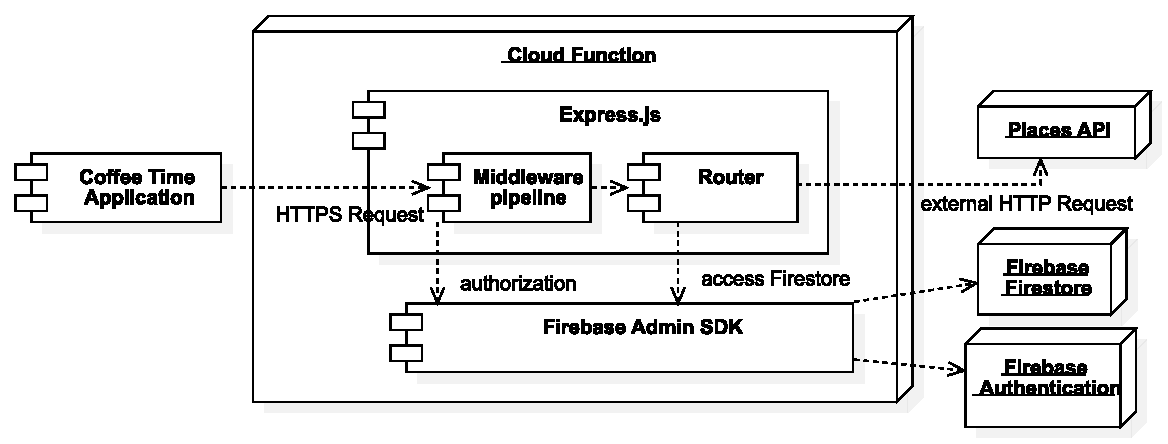
\includegraphics[width=\linewidth]{img/implementation/coffee-api-components.pdf}
    \caption{API Components.}
    \label{fig:cta-relations}
\end{figure}

\subsection{Functions Deployment}
Developer can run functions locally and serve them through localhost while developing them. Once the code is ready, it has to be deployed to the Firebase Cloud Functions service. In order to do that, \textit{Firebase CLI} tooling and its deploy command have to be used. If a~version exists already in the~Firebase, it is replaced by a new one.

Firebase Cloud Functions can be deployed to different physical areas such as \textit{West Europe} or \textit{US East}. While the Coffee Time application is mainly tested in the Czech Republic, \textit{West Europe} was selected as the best option because of its closest availability. One downside is that each location is part of the~API~URL. This can add complexity to the~client side if more locations are used in case of globally available application. 

% ----- % ----- % ----- % ----- % ----- % ----- % ----- % ----- % ----- % ----- % ----- % ----- % ----- % ----- %
\section{Coffee Time}
For Coffee Time purposes, the architecture was slightly simplified and is made from three layers -- domain, data and presentation. The domain layer encapsulates all domain entities and defines contracts for repositories. This layer corresponds with ``Entity'' layer from Clean Architecture. Next, the Data layer encapsulates all external communication such as API requests or location services. This layer also defines data models which are passed down to the repositories where data are processed and transformed to domain entities. Data layer corresponds with \textit{Interface Adapters}. The presentation layer is responsible for describing the user interface and interacts with \gls{bloc} objects where the business logic is encapsulated.

This section describes each layer -- its implementation details and how it is used with other layers.  
% --- # --- # --- # --- # --- # --- # --- # --- # --- # --- # --- # --- # --- # --- # --- # --- # --- # --- #
\subsection{Domain Layer}
Domain Layer defines every entity used by the application, definition of repository contracts -- repository interface definitions and application-wide exceptions. Repository implementation resides in Data layer. 

One of important requirements of the Presentation layer and overall Flutter's philosophy is immutability. Hence, the domain entities are designed as immutable objects. Another requirement is object equality. By default, Dart compare objects by identity -- two objects are same instance, they are considered as identical (equal). In order to have fully functional application, it is necessary to override default equality behaviour to comparison by object properties. 

\subsubsection{Equatable Package}
If the default equality behaviour has to be changed, the \verb|==| operator and \verb|hashCode| getter have to be overridden~\cite{dart-equality}.
Even with small classes, this work becomes quickly tedious and can leads to unnecessary bugs for example when some property is added and developer forgot to update these overrides. Therefore in case of complex classes the amount of bugs only increases. 

\textit{Equatable} package~\cite{package-equatable} (developed by \textit{F. Angelov}) was created to simplify creating immutable classes with proper equality implementation. Class which needs to implement equality has to extend \verb|Equatable| base class provided by the package. Then it is needed to override \verb|props| getter where all class properties are listed. With that setup, equatable package internally provides proper equality comparison. This package is used to for all entities and classes which needed proper equality implementation. An example of its usage is shown in~\Cref{listing:ct-opening-hour-entity}, which is \verb|OpeningHours| entity implementation. 

\begin{listing}[ht]
\begin{minted}{dart}
class OpeningHours extends Equatable {
  final bool openNow;
  final List<Period> periods;
  final List<String> weekdayText;

  OpeningHours({this.openNow, this.periods, this.weekdayText});

  OpeningHours copyWith(
      {bool openNow, List<Period> periods, List<String> weekdayText}) {
    return OpeningHours(
        openNow: openNow ?? this.openNow,
        periods: periods ?? this.periods,
        weekdayText: weekdayText ?? this.weekdayText);
  }

  @override
  List<Object> get props => [openNow, periods, weekdayText];
}
\end{minted}
\caption{OpeningHour Entity with Equality.}
\label{listing:ct-opening-hour-entity}
\end{listing}

\subsubsection{Repositories Contracts}
Domain Layer also defines repository contracts. The repository is used to as connection between presentation layer and data layer. Coffee Time application defines two repositories -- \verb|CafeRepository| and \verb|TagRepository|. Within domain layer, repositories are defined as abstract classes which define required interface. The implementation itself, as was said earlier, is in the data layer. The \verb|CafeRepository|~(\Cref{fig:ct-cafe-repo-interface}) has methods related to cafe places such as finding nearby cafes or user's favorited cafes. 

\begin{figure}[ht]
    \centering
    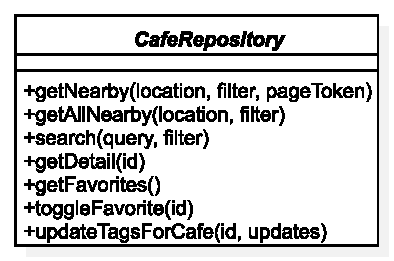
\includegraphics[width=0.5\linewidth]{img/implementation/cafe_repository_interface.pdf}
    \caption{Cafe Repository Interface.}
    \label{fig:ct-cafe-repo-interface}
\end{figure}

\verb|TagRepository|~(\Cref{fig:ct-tag-repo-interface}) has methods related to tags such as getting all available tags or tags assigned to specific cafe. 

\begin{figure}[ht]
    \centering
    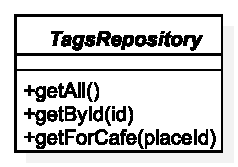
\includegraphics[width=0.33\linewidth]{img/implementation/tag_repository_interface.pdf}
    \caption{Tag Repository Interface.}
    \label{fig:ct-tag-repo-interface}
\end{figure}

In order to have convenient approach of handling exceptions raised within repository (or from layers above) in repository layer, each method of repository returns type \verb|Either<L,R>|. Either is functional concept~\cite{ibm-either} of returning two distinct values from one method. It is used to return desired return type in case of success or error in case of exception. This approach helps to avoid \verb|try - catch| clauses in presentation layer and the code is more readable in functional way. 

The \verb|Either<L,R>| is generic class, where \verb|L| is left type and \verb|R| is right type. The returned value from such method can be used with \verb|when()| or \verb|map()| methods to access actual returned value. Internally the \verb|Either<L,R>| is implemented with \textit{freezed} package~\cite{package-freezed}. This package and its usage is more precisely described later, in the presentation layer. In this way, Either is strongly typed. Similar approach could be use for example \verb|Tuple<T1,T2>| type, but losing strongly typed solution. 

\begin{listing}[ht]
\begin{minted}{dart}
@override
Future<Either<List<Tag>, Failure>> getAll() async {
    try {
      final tags = await _getAllTags();
      return Left(tags); // Return Left type - List<Tag>
    } on ApiException catch (e) {
      // Return Right type - Failure
      return Right(ServiceFailure(errorMsg, inner: e));
    } catch (e) {
      // Return Right type - Failure
      return Right(CommonFailure(e));
    }
}
\end{minted}
\caption{Returning Value as Either within Tag Repository.}
\label{listing:ct-either-repo}
\end{listing}

\Cref{listing:ct-either-repo} shows how \verb|Either<L,R>| is used within \verb|TagRepository|. In case of successful operation, \verb|Left| type is returned, in this case the list of tags. If any exception occurs, the \verb|Right| type -- Failure is returned instead. The usage of such returned value is shown in~\Cref{listing:ct-either-usage}, where either \verb|List<Tag>| is returned or \verb|Failure| object instead.   

\begin{listing}[ht]
\begin{minted}{dart}
// ... call to TagRepository
final result = await repository.getAll();
final allTags = result.when(
      // successful call - get tags
      left: (tags) => tags,
      // failure - return empty array in this case
      // ... and for example log the failure to logger
      right: (failure) => <Tag>[], 
);
\end{minted}
\caption{Usage of Either Returned Value.}
\label{listing:ct-either-usage}
\end{listing}

% --- # --- # --- # --- # --- # --- # --- # --- # --- # --- # --- # --- # --- # --- # --- # --- # --- # --- #
\subsection{Data Layer}
Purpose of layer service is to implement repositories, add services which communicates with Coffee Time API and define a models which are mapped to the responses from API. As with the repositories, the services are implemented against interfaces. This approach helps to write testable code. Repositories which use these services depend on interfaces and not on the concrete implementations. \Cref{fig:ct-repo-services} shows association between repositories and those services. 

\begin{figure}[ht]
    \centering
    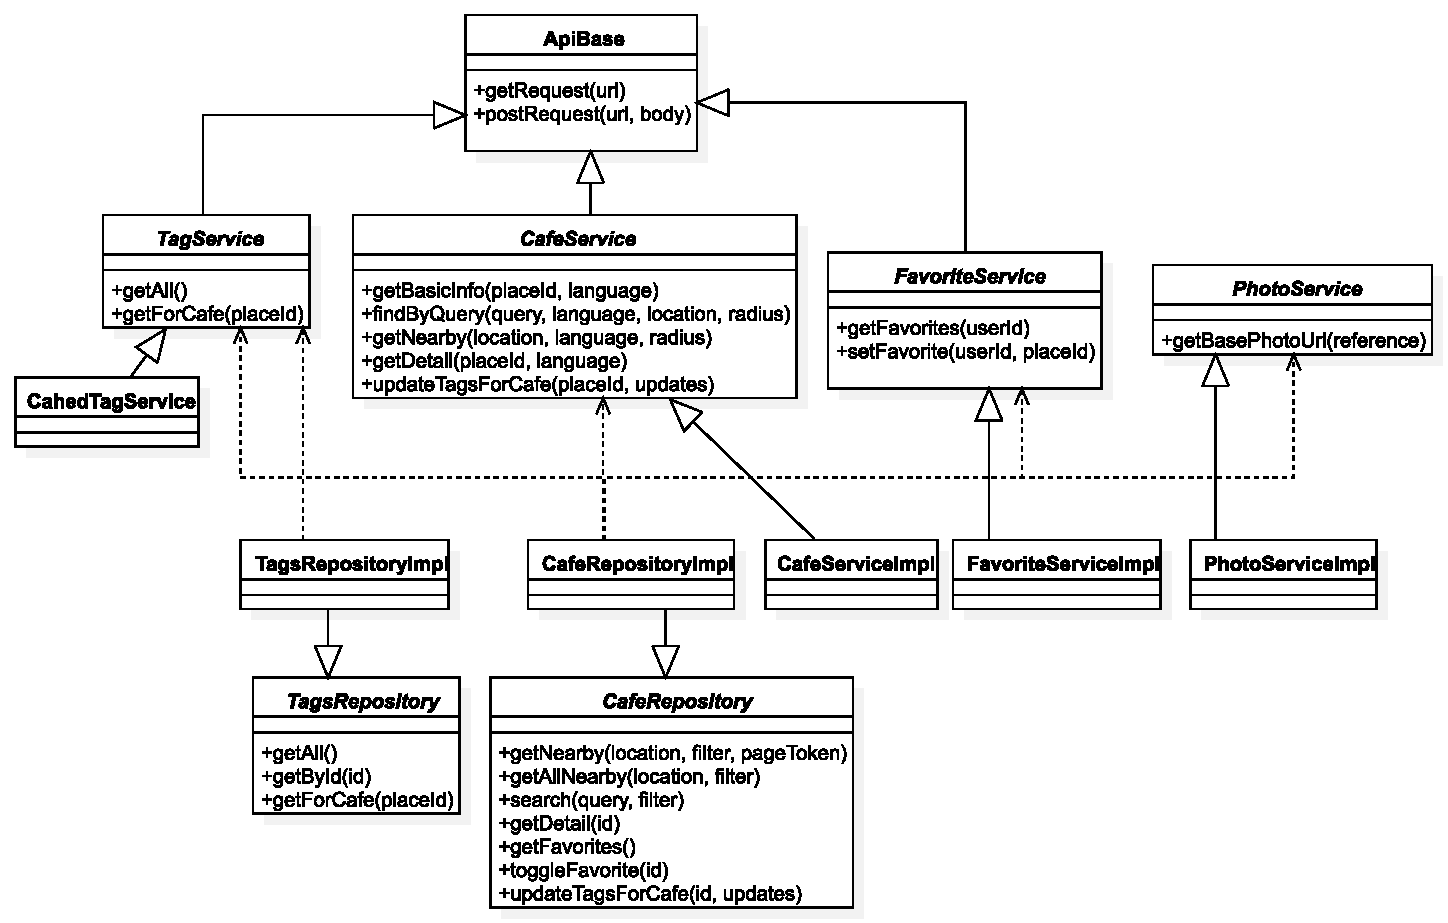
\includegraphics[width=\textwidth]{img/implementation/repo-services.pdf}
    \caption{Repositories and Services Association.}
    \label{fig:ct-repo-services}
\end{figure}

Each service communicates with a concrete part of the Coffee Time API. The~\verb|CafeService| has methods related to obtaining nearby cafes or getting cafe detail, \verb|FavoriteService| has methods to obtain favorited cafes, \verb|PhotoService| gives access to downloading cafe's photos and \verb|TagServices| server for manipulation with tags. 

\subsubsection{Favorite Local Service}
Current application version uses for saving user's favorite cafes only local storage. Thanks to implementation against interface, in the future, the synchronization of favorited cafes over API can be added without breaking other parts of the~application. 

\subsubsection{Cached Tag Service}
To prevent unnecessary amount of calls to API when obtaining all tags, a caching mechanism was implemented for \textit{Tag Service}. When all tags are returned from the API, they are cached for future calls. As a whole implementation is focused on clean code implementation, maintainbality and testability, a generic \verb|CachedValue<T>| class was implemented as wrapper around cachable values. 

\begin{listing}[ht]
\begin{minted}{dart}
typedef ExpirationCallBack<T> = Future<T> Function();

class CachedValue<T> {
  T _value;
  DateTime _timeStored;
  final Duration durability;
  final ExpirationCallBack<T> onExpire;
  final TimeProvider timeProvider;
  // ... constructor ommitted
  Future<T> get() async {
    if (_value == null ||
        timeProvider.now()
                    .difference(_timeStored)
                    .inMilliseconds 
            > durability.inMilliseconds) {
      _value = await onExpire();
      _timeStored = timeProvider.now();
    }
    return _value;
  }
}
\end{minted}
\caption{Cached Value.}
\label{listing:ct-cached-value}
\end{listing}

The \verb|CachedValue| accepts \verb|TimeProvider| which provides current time, duration for how long value should be cached and \verb|ExpirationCallback<T>| which is called whenever cached value has to be re-assigned. \verb|TimeProvider| class is abstraction of \verb|DateTime.now()|. This abstraction was necessary for unit testing.   

\subsubsection{Entity Models}
Every response from API which contains data is mapped to \textit{model}. Model is a immutable class, similar to \textit{entity} classes except that model includes parsing from (and to) JSON format. These models are returned by services to repositories, where models are transformed into entities and returned further. Subset of models correspond with entities in one to one relationship, some other models have logic for mapping its values to the corresponding entity. 
% --- # --- # --- # --- # --- # --- # --- # --- # --- # --- # --- # --- # --- # --- # --- # --- # --- # --- #
\subsection{Representation Layer}
The responsibility of representation layer is define user interface, connect it with BLoCs objects which communicate with repositories. How to properly organize and architect user interface within Flutter, mainly how to separate responsibilities between \gls{bloc} classes is still very subjective opinion and there is no ``best practice'' yet. However, commonly used approach is divide \gls{bloc} responsibility per ``big enough feature''. That means, identify feature of the application and separate \gls{bloc} responsibilities appropriately. Another approach is ``\gls{bloc} per screen''. This approach is well suited for smaller application. As the Coffee Time is still smaller application, second approach was chosen. Each screen has its own, separated \gls{bloc} class. Each \gls{bloc} defines states for given screen and set of events which can accept.  

\begin{figure}[ht]
	\dirtree{%
		.1 core \DTcomment{shared BLoCs}.
		.1 screens.
		.2 cafe\_list \DTcomment{Cafe List Screen}.
		.3 bloc \DTcomment{Cafe List's BLoC}.
		.4 bloc.dart \DTcomment{BLoC implementation}.
		.4 state.dart \DTcomment{BLoC's states}.
		.4 event.dart \DTcomment{BLoC's events}.
		.3 widgets \DTcomment{Specific screen widgets}.
		.3 screen.dart \DTcomment{Main screen widget}.
		.2 detail \DTcomment{Next screen}.
		.2 ...
		.1 shared \DTcomment{Shared widgets and theming}.
		.1 app.dart \DTcomment{Main application widget}.
	}
    \caption{Presentation Layer Screens Organization.}
    \label{fig:ct-pres-organis}
\end{figure}

\Cref{fig:ct-pres-organis} shows overall presentation code organisation. Each screen has defined entry file \verb|screen.dart| where screen's widget is defined. Widgets folder contains all screen specific widgets. Bloc folder contains BLoC implementation along with states and events. Shared folder contains shared widget and application theming related settings. This organization helps to keep organized code with strictly defined where particular \gls{bloc} can be found for given screen. 

\subsubsection{Flutter\_bloc Package}
As was pointed out in the first chapter, \textit{flutter\_bloc} is a package developed to help implement a~\gls{bloc} pattern with a~simplified manner. Each \gls{bloc} class has to extend \verb|BLoC<TEvent,TState>| class. Its simple usage was shown in~\Cref{listing:counter-bloc-bloc} in the~first chapter. Each \gls{bloc} class has to override \\ \verb|mapEventToState(TEvent)| method. In this method, \gls{bloc} should decide which state to yield based on the event. When state is yielded, it is compared to current \gls{bloc}'s state and if they are different, widgets listening for changes are rebuilt. This implies important requirement for state class -- it has to have overridden equality comparison. 

To connect \gls{bloc} with other widgets, \textit{flutter\_bloc} offer several widgets to help that:

\begin{itemize}
    \item \textbf{BlocProvider} -- Provides \gls{bloc} instance down to the tree. Internally it is using \textit{Provider} package.
    \item \textbf{BlocBuilder\textless Bloc, State\textgreater} -- Listen for changes from given Bloc and its state, which has to be provided somewhere in the parent widgets. Widget has \textit{builder} callback, where new widget based on obtained state is returned. 
    \item \textbf{BlocListener\textless Bloc, State\textgreater} -- In order to do side effects, such as display notification, \textit{BlocListener} can be used. As \textit{BlocBuilder} is is listening for changes from Bloc and its new state. 
    \item \textbf{BlocConsumer\textless Bloc,State\textgreater} -- Combines functionality of \textit{BlocBuilder} and \textit{BlocListener} together.
\end{itemize}

\subsubsection{State and Events Implementation}
Each \gls{bloc} has typically more than one state and event. To do that, the simplest approach is to define abstract class for state (event) and every specific state (event) extends this abstract class. This works well, however in the \verb|mapEventToState()| method with this approach has to be distinguished between specific types. Only one possible option is to use \verb|is| operator. Such example is shown in~\Cref{listing:ct-state-map-abstract}. 

\begin{listing}[ht]
\begin{minted}{dart}
Stream<CafeListState> mapEventToState(CafeListEvent event) async* {
    if (event is LoadNext) {
      yield* _mapLoadNext(event);
    } else if (event is Refresh) {
      yield* _mapRefresh(event);
    } else if (event is SetFavorite) {
      yield* _mapSetFavorite(event);
    } else if (event is UpdateTags) {
      yield* _mapUpdateTags(event);
}
\end{minted}
\caption{Abstract Class Approach -- State Mapping to Events.}
\label{listing:ct-state-map-abstract}
\end{listing}

This approach has several issues, mainly: 

\begin{itemize}
    \item Repetitive code with ``event is'' and,
    \item no compile time control. When new event is added, there is no way to force add new ``else if'' branch. Options such as default else with throwing exception is not viable solution, as it does not add any benefit.
\end{itemize}

Same issue is with mapping states within widgets. There is better solution with ``union types'' and functional way of ``map'' method.

\subsubsection{Union Types to the Rescue}
Union is an object containing value of different types, but allows manipulating that value with type-safety and compile time check. In fact, earlier introduced \verb|Either<L,R>| is a such union type. Package \textit{Freezed}~\cite{package-freezed}, by the same author of the \textit{Provider}, helps to do such implementation. 

One popular functionality within \textit{Dart} ecosystem is code-generation and \textit{Freezed} package is no difference. In order to implement Union type, developer has to define abstract class with all possible sub-values and package will generate rest of the code. The generated class is immutable and has:

\begin{itemize}
    \item overridden equality operators,
    \item \verb|copyWith()| method to copy object with altered properties, 
    \item \verb|map()| method to map from one possible sub-class,
    \item \verb|when()| method to map from one possible value. Difference with \verb|map()|  is that when returns values of the sub-class, but \verb|map()| returns sub-class instance,
    \item and has \verb|maybeMap()| and \verb|maybeWhen()| which do not force include all possible values. 
\end{itemize}

\begin{listing}[ht]
\begin{minted}{dart}
@freezed
abstract class CafeListEvent with _$CafeListEvent {
  const factory CafeListEvent.loadNext(
      {String pageToken, 
       @Default(Filter()) Filter filter}) = LoadNext;
  const factory CafeListEvent.refresh(
          {@Default(Filter()) Filter filter}) = Refresh;
  const factory CafeListEvent.setFavorite(
      {@required String cafeId, 
       @required bool isFavorite}) = SetFavorite;
  const factory CafeListEvent.updateTags(
      {@required String cafeId,
      @required List<TagReputation> tags}) = UpdateTags;
}
\end{minted}
\caption{Union Class Approach -- CafeList Event Definition.}
\label{listing:ct-event-union}
\end{listing}

\begin{listing}[ht]
\begin{minted}{dart}
@override
Stream<CafeListState> mapEventToState(CafeListEvent event) async* {
    yield* event.map(
      loadNext: _mapLoadNext,
      refresh: _mapRefresh,
      setFavorite: _mapSetFavorite,
      updateTags: _mapUpdateTags,
    );
}
\end{minted}
\caption{Union Class Approach -- Events Mapping To State.}
\label{listing:ct-event-union-usage}
\end{listing}

Union type forces compile-time check in case of \verb|map()| usage. This eliminate issue with \verb|is| operator. \Cref{listing:ct-event-union} shows \textit{CafeListEvent} definition as union type. In~\Cref{listing:ct-event-union-usage} is shown same event mapping to state but with union approach. Whenever new event is added, the compile-time error will occur as the \verb|map()| forces it.

Similarly state mapping within CafeList Screen~(\Cref{listing:ct-state-cafe-list-union-usage}) is simplified and compile-time safe. 

\begin{listing}[ht!]
\begin{minted}{dart}
return BlocBuilder<CafeListBloc, CafeListState>(
  builder: (context, state) {
    return state.map(
      loading: (_) => const CircularLoader(),
      loaded: (loaded) {
        if (loaded.cafes.length == 0) {
          return const NoData();
        }
        return CafeList(state: loaded);
      },
      failure: (failure) => FailureContainer(
        message: failure.message,
        onRefresh: () => context
            .bloc<CafeListBloc>()
            .add(Refresh(filter: failure.filter)),
      ),
      // shortened for brevity
    );
  },
);
\end{minted}
\caption{CafeListState Mapping within CafeList Screen Build Method.}
\label{listing:ct-state-cafe-list-union-usage}
\end{listing}

\subsubsection{BLoC to BLoC Communication}
Each screen has its own assigned \gls{bloc}, however some communication between BLoCs is also needed. For example in case of updating favorite cafe, the~\textit{FavoriteBloc} is updated. The\textit{ CafeListBloc} and \textit{DetailBloc} listen to such changes and updates appropriately. \Cref{fig:ct-screens-bloc} shows associations between screens, blocs and, bloc to bloc communication.

\begin{figure}[h!]
    \centering
    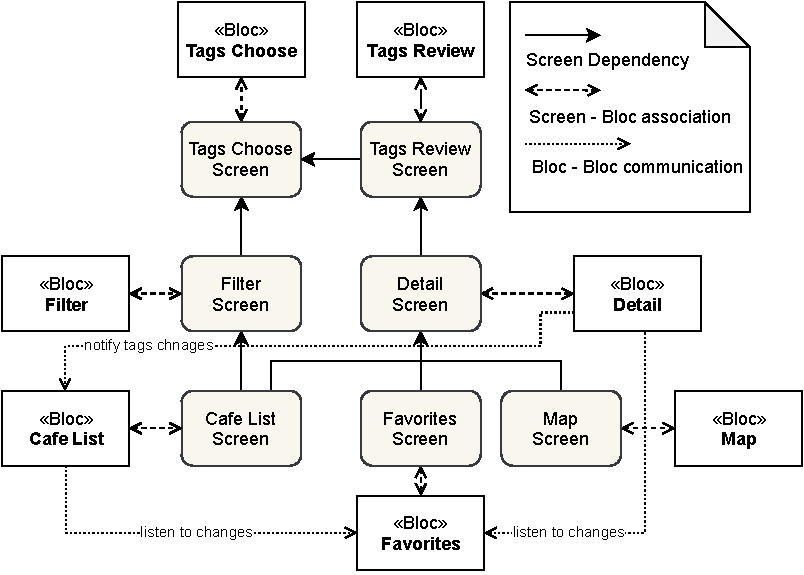
\includegraphics[width=\textwidth]{img/implementation/bloc-screens-dependencies.pdf}
    \caption{Screens and Blocs Association.}
    \label{fig:ct-screens-bloc}
\end{figure}

\section{SOLID and Dependency Injection}
One important part of maintainable and testable code are \textit{SOLID} principles, originally designed by \textit{Bob C. Martin}~\cite{bob-martin-design-patterns}. Each letter stands for one principle: 

\begin{enumerate}
    \item Single Responsibility Principle -- a class should only have on responsibility. That class should have one reason to change.
    \item Open Closed Principle -- a class should be open for extension, but closed for modification. 
    \item Liskov Substitution Principle -- if class A is a subtype of class B, then it should be possible to replace B with A without disrupting the behaviour of the program. 
    \item Interface Segregation -- many specific interfaces are better than one general-purpose interface. In other words, split larger interfaces to smaller ones. 
    \item Dependency Inversion -- high-level modules should not depend on low-level modules. Both should depend on abstractions.
\end{enumerate}

Each class (module) within Coffee Time Application, such as repository, service or \gls{bloc} which depends on some other classes, depends on abstractions. These dependencies lists as required in class constructor. Dependency Injection mechanism is used to provide concrete implementations of each required abstraction to classes which depends on it. 

Dart (and Flutter) does not provide such Dependency Injection mechanism out of the box. However, \textit{get\_it} is a package, which helps with that. In fact, \textit{get\_it} works more as Service Locator. Every concrete implementation has to be registered and paired with its abstraction counterpart within \textit{GetIt} container. When those implementation are registered, container can be accessed through singleton instance and obtain concrete implementation.

However, such Service Locator is usually considered as anti-pattern if used careless. If such container is accessed everywhere, it can hides dependencies and it is highly coupled to every module. On the other hand, if each module lists its dependencies within constructor, such modules can be constructed at one place. In this place, usually called ``composition root'', this issue can be avoided. Thus, in the Coffee Time implementation, every dependency is registered within \textit{GetIt} container (see \verb|di_container.dart| file). Then concrete implementations are created through \textit{GetIt} locator mainly in \verb|App.dart| or when doing navigation between screens. 

\section{Unit Testing}
Properly written project should have tested code. Coffee Time application has written unit tests for each layer. Domain entities has unit tests for their logic, service has unit tests for proper handling of API communication, repositories has tests for business logic and, \gls{bloc}s are tested that emits proper state based on received events. 

In order to have independent, isolated unit tests, some class dependencies are mocked to provides desired behaviour. To create mocks, a \textit{mockito} package~\cite{package-mockito} is used. Package offers flexible of mocking parts of the class. Developers can define what mocked method for given parameters should respond. Another package, \textit{bloc\_test}~\cite{package-bloctest} (same author of \textit{Equatable} and \textit{flutter\_bloc} packages) is used to test implementation of BLoCs. 

An example of unit test is shown in~\Cref{listing:ct-filter-bloc-unit-tests}. Unit tests use both mentioned packages. \verb|FilterBloc| has dependency on \verb|TagRepository| which is mocked in order to return faked values. Method \verb|blocTest()| comes from second packages and offer convenient way for \gls{bloc} testing. 

\begin{listing}[ht]
\begin{minted}{dart}
// creates mocked TagRepository
class MockTagRepository extends Mock 
                        implements TagRepository {}

void main() {
  MockTagRepository tagRepository;
  final allTags = [
    Tag(id: '1', icon: Icons.filter, title: '1'),
    Tag(id: '2', icon: Icons.filter, title: '2'),
  ];

  setUp(() {
    tagRepository = MockTagRepository();
    // when getAll called on repository
    // then answer with defined allTags array
    when(tagRepository.getAll())
         .thenAnswer((_) async => Left(allTags));
  });

  FilterBloc createBloc(Filter filter) =>
      FilterBloc(tagRepository: tagRepository, 
                 initialFilter: filter);
  
  blocTest(
    'Remove tag and should be empty',
    build: () async => createBloc(Filter(tagIds: ['1'])),
    act: (bloc) async {
      bloc.add(Init());
      bloc.add(RemoveTag(tagId: '1'));
    },
    expect: [
      isA<FilterBlocState>(),
      FilterBlocState(
          filter: Filter(tagIds: []), 
          addedTags: [], 
          notAddedTags: allTags
       ),
    ],
  );
   // ...
}
\end{minted}
\caption{FilterBloc Unit Tests.}
\label{listing:ct-filter-bloc-unit-tests}
\end{listing}

\section{Conclusion}
This chapter described important parts of the implementation. In the beginning, the design and the used framework for Coffee Time API implementation along with the deployment to Cloud Functions were represented. Furthermore the architecture of the application, each architecture's layer and used techniques were discussed. In the following chapter, a development process with continuous integration is described along with internal testing and final user testing before release.